\clearpage
\section{Funktionsweise}\label{sec:Funktionsweise}
Folglich soll die Funktionsweise einer differenziellen Kryptoanalyse auf eine Runde vom Data Encryption Standard (DES) erläutert werden (Es wird nur die rechte Seite einer DES-Runde betrachtet). 
Wie der Name es schon andeutet, wird bei diesem Verfahren die Differenz aus zwei Klartexten, in diesem Beispiel mit $P_{1}$ und $P_{2}$ bezeichnet, verwendet. Die Differenz wird üblicherweise mit $P'$ bezeichnet und folgt aus einer XOR-Verknüpfung der Klartexte, also $P' = P_{1} \oplus P_{2}$.
Funktionen wie Expansionen, Permutationen oder XOR-Verknüpfen haben keine Einfluss auf die Differenz der Texte. Die Differenz kann also fast durch die gesamte Feistelstruktur beobachtet werden. Die Abbildung \ref{fig:DES_Differenz} zeigt wie sich eine Differenz durch das Netzwerk verhält. 

\begin{figure}[h]
	\centering
	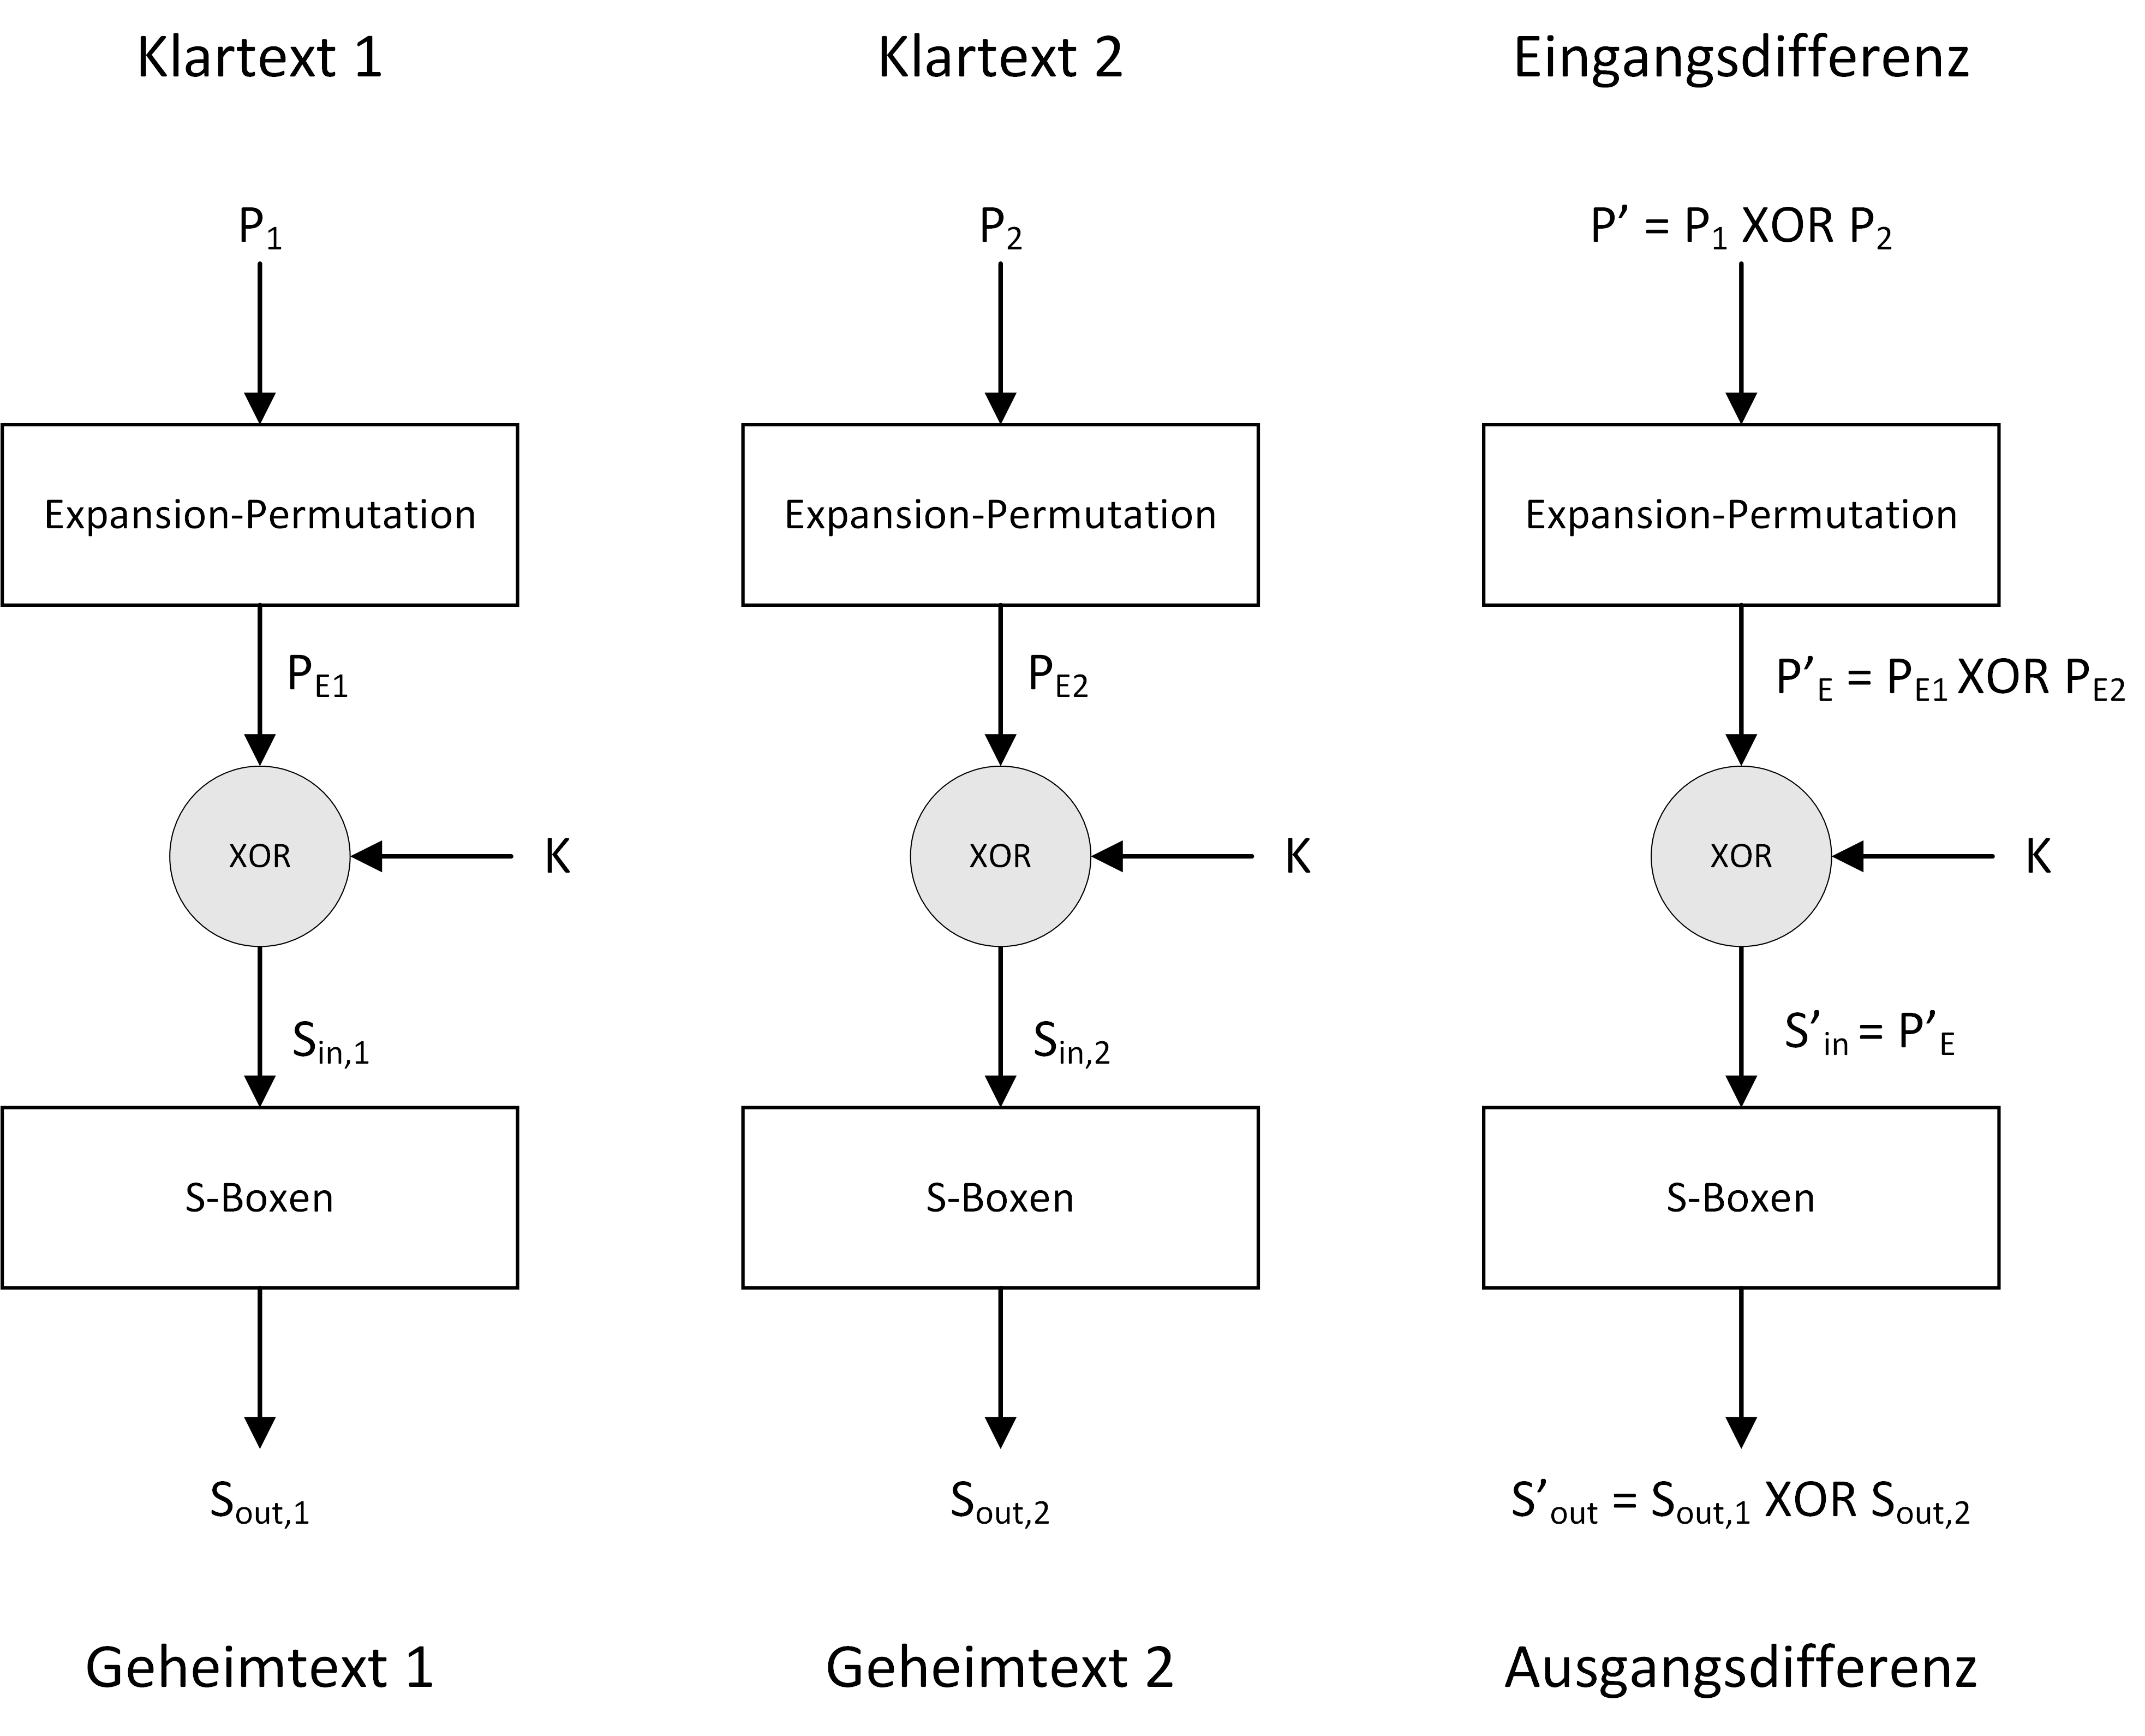
\includegraphics[width=1.0\linewidth]{graphics/DES_Differenz.jpg}
	\caption{Verhalten von Klartext 1, 2 und der Differenz davon durch die Feistelstruktur einer Runde von DES \cite{the_morpheus_tutoials_kryptographie_2016}}
	\label{fig:DES_Differenz}
\end{figure}

Die Eingangswerte $S_{in,1}$ und $S_{in,2}$ der S-Boxen sind ohne Schlüssel nicht bekannt. Bei der Spalte \glqq Differenz\grqq{} ist dieser Eingang $S'_{in}$ aber bekannt. Eine doppelte XOR-Verknüpfung mit dem Schlüssel aufhebt sich auf. Mit anderen Worten ist: 

\begin{equation}\label{equ:Schluessel_Differenz}
S'_{in} = S_{in,1} \oplus S_{in,2} = (P_{E,1} \oplus K) \oplus (P_{E,2} \oplus K) = P_{E,1} \oplus P_{E,2} = P'_{E} 
\end{equation}


Mit dieser Eigenschaft können die S-Boxen genauer analysiert werden. 
Wie bereits in der Einleitung erwähnt, sind die S-Boxen nicht-lineraren Funktion. Um diese zu umgehen kann mit Wahrscheinlichkeiten gearbeitet werden.
Anhand der öffentlich zugänglichen S-Boxen kann eine Differenzenverteilungstabelle aufgestellt werden. In dieser wird für jede Eingangsdifferenz die Zahl Wertepaar gegeben welche eine bestimmte Ausgangsdifferenz erzeugen. 
Es gibt bei DES $2^{6} = 64$ verschieden mögliche Eingangsdifferenzen pro S-Box. Jede Eingangsdifferenz kann mit 64 verschiedenen Wertepaare erzeugt werden. Als Beispiel: für eine Eingangsdifferenz von $34_{h}$ (Hexadezimalzahl) gibt es laut Differenzenverteilungstabelle nur zwei von den 64 Wertepaar die, beim Durchqueren der S-Boxen 1, eine Ausgangsdifferenz von $04_{h}$ erzeugen \cite{noauthor_differenzielle_2019}\cite{biham_differential_1990}. 

Da bei einer chosen plaintext attack die Ausgangsdifferenz bekannt ist, können die möglichen Eingangswertepaare $(S_{in,1}, S_{in,2})$ in einer weiteren Tabelle abgelesen werden. Entsprechend der Differenzenverteilungstabelle gibt es mehr oder weniger solche möglichen Eingangspaar.
Für das Beispiel mit der Eingangsdifferenz $34_{h}$ und der Ausgangsdifferenz $04_{h}$ gibt es die 2 Wertepaare $(S_{in,1}, S_{in,2}) = (13_{h}, 27_{h})$ oder $(S_{in,1},S_{in,2}) = (27_{h}, 13_{h})$. Wäre die Ausgangsdifferenz $02_{h}$ bei einer Eingangsdifferenz von $34_{h}$ würde es 16 mögliche Wertepaare geben. 

Da nun die Eingangswerte bekannt sind, kann der Schlüssel wie folgt berechnet werden:
\begin{equation}\label{equ:Schluessel_Loesung}
K = P_{E,1} \oplus S_{in,1} = P_{E,2} \oplus S_{in,2}
\end{equation}

Weil nicht mit Sicherheit gesagt werden kann welches Wertepaar $(S_{in,1}, S_{in,2})$ das richtige ist, gibt es bei diesem Beispiel zwei mögliche Schlüssel. Es müssten die anderen S-Boxen betrachtet oder mehrere Durchgänge durchgeführt werden, um den falschen Schlüssel auszuschliessen. 














